\section{Einleitung}

\subsection{Motivation und Problemstellung}
In der heutigen Zeit erweist sich Flexibilität als eine immer bedeutendere Determinante für den Erfolg von Unternehmen. So müssen diese stets in der Lage sein, sich effizient an verändernde Marktbedingungen anzupassen. Unternehmen sehen sich deshalb vornehmlich damit konfrontiert, die in Enterprise-Ressource-Planning-Systemen (\acs{ERP}-Systemen) abgebildeten Prozesse auf externe Einflüsse, wie Kundenbedürfnisse, rechtliche Vorschriften und neue Technologien auszurichten. Mit der \textit{Composable-Enterprise-Architektur (CEA)} hat sich in den vergangenen Jahren ein Konzept etabliert, welches Unternehmen bei der Bewältigung dieser Disruptionen unterstützen soll. Die CEA ist ein IT-Konzept, welches Unternehmen ermöglicht, Systeme aus modularen wiederverwendbaren Software-Kompo\-nenten zusammenzusetzen \cite{.20230313}. Laut Martin Henning, Head of New Ventures and Technologies bei der SAP, sind Unternehmen mit diesem Architekturkonzept nicht länger auf \enquote{rigide ERP-Software} angewiesen, sondern vielmehr in der Lage, Geschäftsprozesse auf Grundlage einzelner Software-Bausteine zu digitalisieren \cite{Galer.20221019}. Bei einer Änderung der Geschäftsanforderungen besteht somit die Möglichkeit, einzelne Software-Kompo\-nenten dynamisch auszutauschen, ohne dass Anpassungen am Gesamtsystem erforderlich sind. Dieser Composable-Trend ist nicht nur bei der SAP, sondern ebenfalls bei anderen Unternehmen erkennbar. So wurde in Gartners Top-Trend-Forschung 2022 prognostiziert, dass bis zum Jahr 2024 80 Prozent der befragten Chief Information Officers (\acs{CIO}s) die modulare Gestaltung von Geschäftsprozessen als eine der fünf wichtigsten Gründe für betriebliches Wachstum betrachten werden \cite{Gartner.20230408}. Um die Geschäftsprozesse in einer CEA noch individueller auf die eigenen Bedürfnisse zuschneiden zu können, neigen Unternehmen dazu, die bestehende Architektur um eigenentwickelte modulare Bausteine zu erweitern. Damit Effizienz und Anpassungs\-fähigkeit vollständig ausgeschöpft werden kann, ist es unerlässlich, dass diese Bausteine schnell bereitgestellt und in das bestehende System integriert werden. Abhilfe schaffen soll dabei die in der Literatur als \textit{\ac{CI/CD}} bekannte Entwicklerpraktik. Damit soll sichergestellt werden, dass Änderungen am Code kontinuierlich und zuverlässig in den Produktionssystemen bereitgestellt werden. Dies kann mithilfe einer CI/CD-Pipeline realisiert werden. Mit dieser ist es möglich, die in einer Entwicklungsabteilung anfallenden Softwarebereitstellungsprozesse vollständig zu automatisieren. Empirische Daten belegen, dass der Einsatz dieser Pipelines den Bereitstellungsprozess im Durchschnitt um das Doppelte beschleunigt, während die Fehlerquote um 50 Prozent reduziert wird \cite{abdalslam.20230128}.\\ 
Da CI/CD-Pipelines eine kontinuierliche Bereitstellung und Integration modularer Software-Komponenten ermöglichen, sind diese insbesondere für die CEA von großer Bedeutung. Um den spezifischen, in einer CEA vorliegenden Bedürfnissen gerecht zu werden, benötigt die Implementierung von CI/CD-Prozessen jedoch im Vergleich zu herkömmlichen System-Architekturen einer differenzierten Herangehensweise. Damit die Unabhängigkeit einzelner Software-Komponenten gewährleistet werden kann, besteht für CEA die Notwendigkeit einer granularen und dezentralen Pipeline-Struktur. Dabei bleibt zu hinterfragen, ob gegenwärtige CI/CD-Tools in der Lage sind, diesen Anforderungen zu genügen.


\subsection{Zielsetzung und Abgrenzung}
Die technische Beratungsabteilung SAP Data Technology Services (\acs{SAP DTS}) unterstützt Kunden bei der Implementierung von ERP-Services auf der Cloud-Plattform \ac{SAP BTP}. Um ihren Kunden optimale Lösun\-gen anzubieten, sind aktuelle Technologieinnovationen für das SAP DTS von hoher Bedeutung. In diesem Kontext stellt ebenfalls die CEA im Bereich Unternehmenssoftware ein hochrelevantes und zukunftsweisendes Thema dar. Neben der Planung, dem Entwurf und der Erstellung von IT-Services berät das SAP DTS Kunden ebenfalls in der Implementierung von Softwarebereitstellungsprozessen. Um diese Vorgänge zu automatisieren, werden von dem SAP DTS i.d.R. drei verschiedene CI/CD-Pipeline-Tools empfohlen. Dazu gehören Azure Pipelines, Jenkins und \acs{SAP CI/CD}. Ziel der Arbeit ist deshalb, zu evaluieren, welches dieser Tools den größten Mehrwert zur Bereitstellung von Cloud-Software für eine CEA liefert. Dafür soll ein Entscheidungs-Framework erstellt werden, anhand dessen eine Bewertung der Lösungen erfolgt. Es besteht die Möglichkeit, dass das mit dem Entscheidungs-Framework erhaltene Resultat nicht auf alle Unternehmen übertragbar ist. Aus diesem Grund ist in der vorliegenden Arbeit ebenfalls vorgesehen, das Ergebnis in einer abschließenden Handlungsempfehlung einzuordnen und zu differenzieren. Daraus resultiert folgende Forschungsfrage:\\
\textit{Welches Tool bietet zur Automatisierung der Bereitstellungsprozesse für Composable-\-Enterprise-Architekturen den größten Mehrwert?}\\
Im Rahmen der Zielsetzung werden folgende Abgrenzungen vorgenommen: Auf der SAP BTP können Anwendungen auf verschiedenen Laufzeitumgebungen betrieben werden. Dafür wird neben Neo und Kyma ebenfalls Cloud Foundry bereitgestellt. In der vorliegenden Arbeit wird dabei jedoch ausschließlich die Bereitstellung von Software in der Cloud-Foundry-Laufzeitumgebung untersucht. Zudem beschränkt sich die Analyse der CI/CD-Tools auf Anwendungen, welche auf den Programmier-Frameworks SAP CAP Node sowie SAP UI5 basieren. Diese Abgrenzung wird gezogen, da das SAP DTS ausschließlich in diesen Technologien berät.  

\subsection{Aufbau der Arbeit}
Im ersten Teil der Arbeit erfolgt eine Definition und Abgrenzung der CEA. In diesem Zusammenhang werden sowohl betriebswirtschaftliche Prinzipien als auch die mit der IT-Architektur herbeigeführten Unternehmenspotenziale veranschaulicht. Im Anschluss werden technologische Konzepte der CEA erläutert. Dabei wird dargelegt, wie Composable-Enterprises (\acs{CE}s) ihre Architektur gestalten müssen, um geschäftlichen Abläufe adäquat in der Unternehmenssoftware abzubilden. Im nachfolgenden Kapitel werden im Rahmen der Softwareentwicklung anfallende Integrations- und Bereitstellungsprozesse beschrieben. Hierbei wird zunächst erläutert, wie die Entwicklungskonzepte \textit{Agile} und \textit{DevOps} zur Optimierung dieser Prozesse beitragen. Daraufhin werden CI/CD-Pipelines, also Tools zur Automatisierung dieser Bereitstellungsprozesse, erläutert. In diesem Kontext werden insbesondere die in der CI/CD-Pipeline abgewickelten Schritte sowie bei der SAP verwendete Tools beschrieben.Im Methodikteil wird das gewählte Vorgehen zu den Experteninterviews, welche zur Erhebung qualitativer Daten durchgeführt werden, erläutert. Des Weiteren wird der \textit{Analytische Hierarchieprozess (\acs{AHP})}, das Instrument zur Bestimmung des optimalen CI/CD-Tools beschrieben. Im Teil der Durchführung erfolgt die Anwendung der Methodik auf die in den Experteninterviews erhobenen Daten. So werden im Rahmen des AHP-Verfahrens Entscheidungskriterien festgelegt und gewichtet. Um eine objektive Evaluierung der CI/CD-Pipeline-Tools zu ermöglichen, werden in diesem Abschnitt ebenfalls Bewertungsmetriken definiert. Im Anschluss werden die zu untersuchenden Entscheidungsalternativen anhand jedes Kriteriums bewertet. Auf dieser Grundlage lässt sich ein aggregierter Nutzwert ermitteln, welcher wiederum zur Identifikation des optimalen CI/CD-Tools beiträgt. 
\begin{center}
	\begin{figure}[H]
		\centering
		\scalebox{0.4}{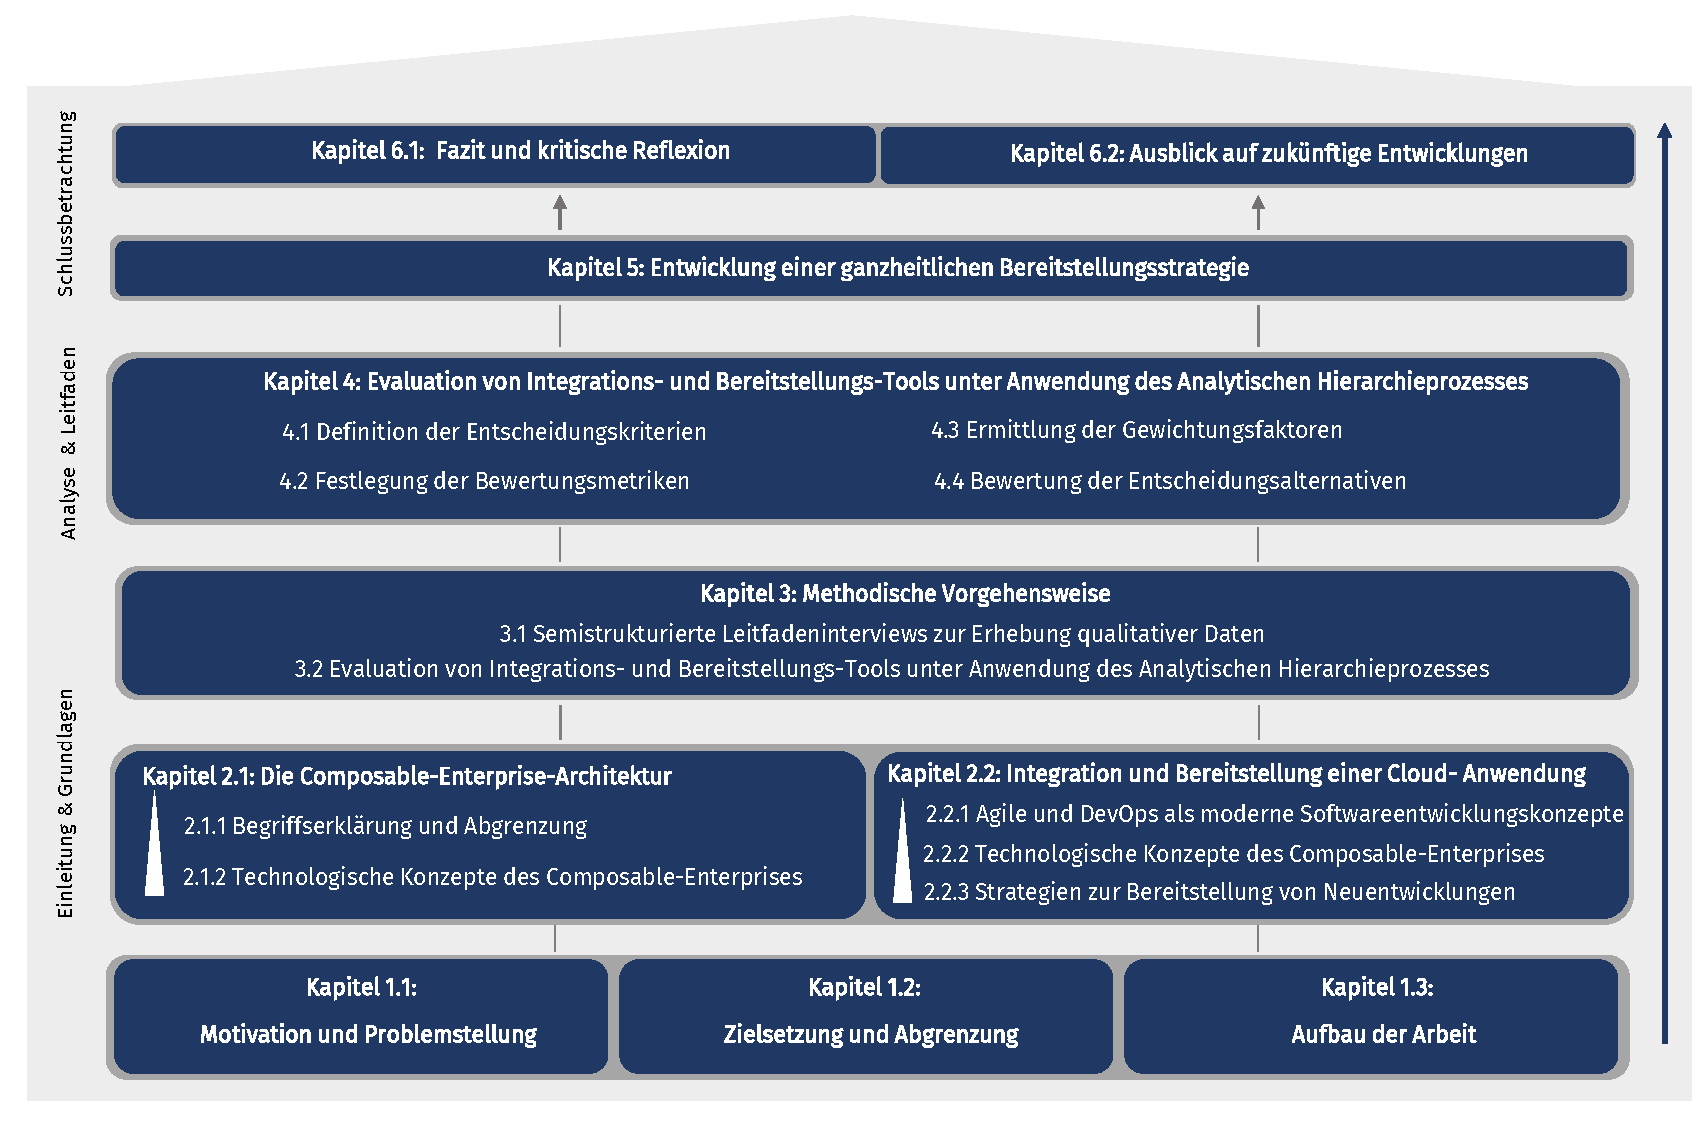
\includegraphics{Aufbau}}
		\caption[Aufbau der Arbeit]{Aufbau der Arbeit. Eigene Darstellung.}
		\label{fig:Aufbau}
	\end{figure}	
\end{center}
\vspace*{-15mm}
In der folgenden Handlungsempfehlung wird eine ganzheitliche Bereitstellungsstrategie für Unternehmen, welche eine CEA implementieren, entwickelt. Dabei wird das Ergebnis des AHP-Verfahrens analysiert und in Abhängigkeit verschiedener Unternehmensstrategien abgegrenzt. Abgerundet wird die Arbeit durch die Zusammenfassung der Erkenntnisse, einer kritischen Beleuchtung des Vorgehens und der Evaluierung zukünftiger Forschungsansätze. 

